\section*{Revisjonshistorie}
\begin{center}
 \begin{tabular}{|p{2.5cm} p{5.5cm}|} 
 \hline
 År & Forfatter \\ [0.5ex] 
 \hline\hline
 2020 & Kolbjørn Austeng\\
 \hline
 2021 & Kiet Tuan Hoang\\
 \hline
 2022 & Kiet Tuan Hoang \\ 
 \hline
 2023 & Kiet Tuan Hoang \\
 2023 & Tord Natlandsmyr \\
 \hline
 2024 & Terje Haugland Jacobsson \\
      & Tord Natlandsmyr \\
 \hline
\end{tabular}
\end{center}

\begin{alphasection}
\section{Introduksjon - Kort om micro:bit}
BBC micro:bit er et lite kort (se figur \ref{fig:micro:bit}) som i utgangspunktet ble utviklet for å skape interesse for programmering hos barn. For å gjøre dette mulig, finnes det et veldig vennlig webgrensesnitt der man kan programmere kortet med programmeringsklosser. 

\begin{figure}[H]
    \centering
    \begin{subfigure}{0.5\textwidth}
    \centering
        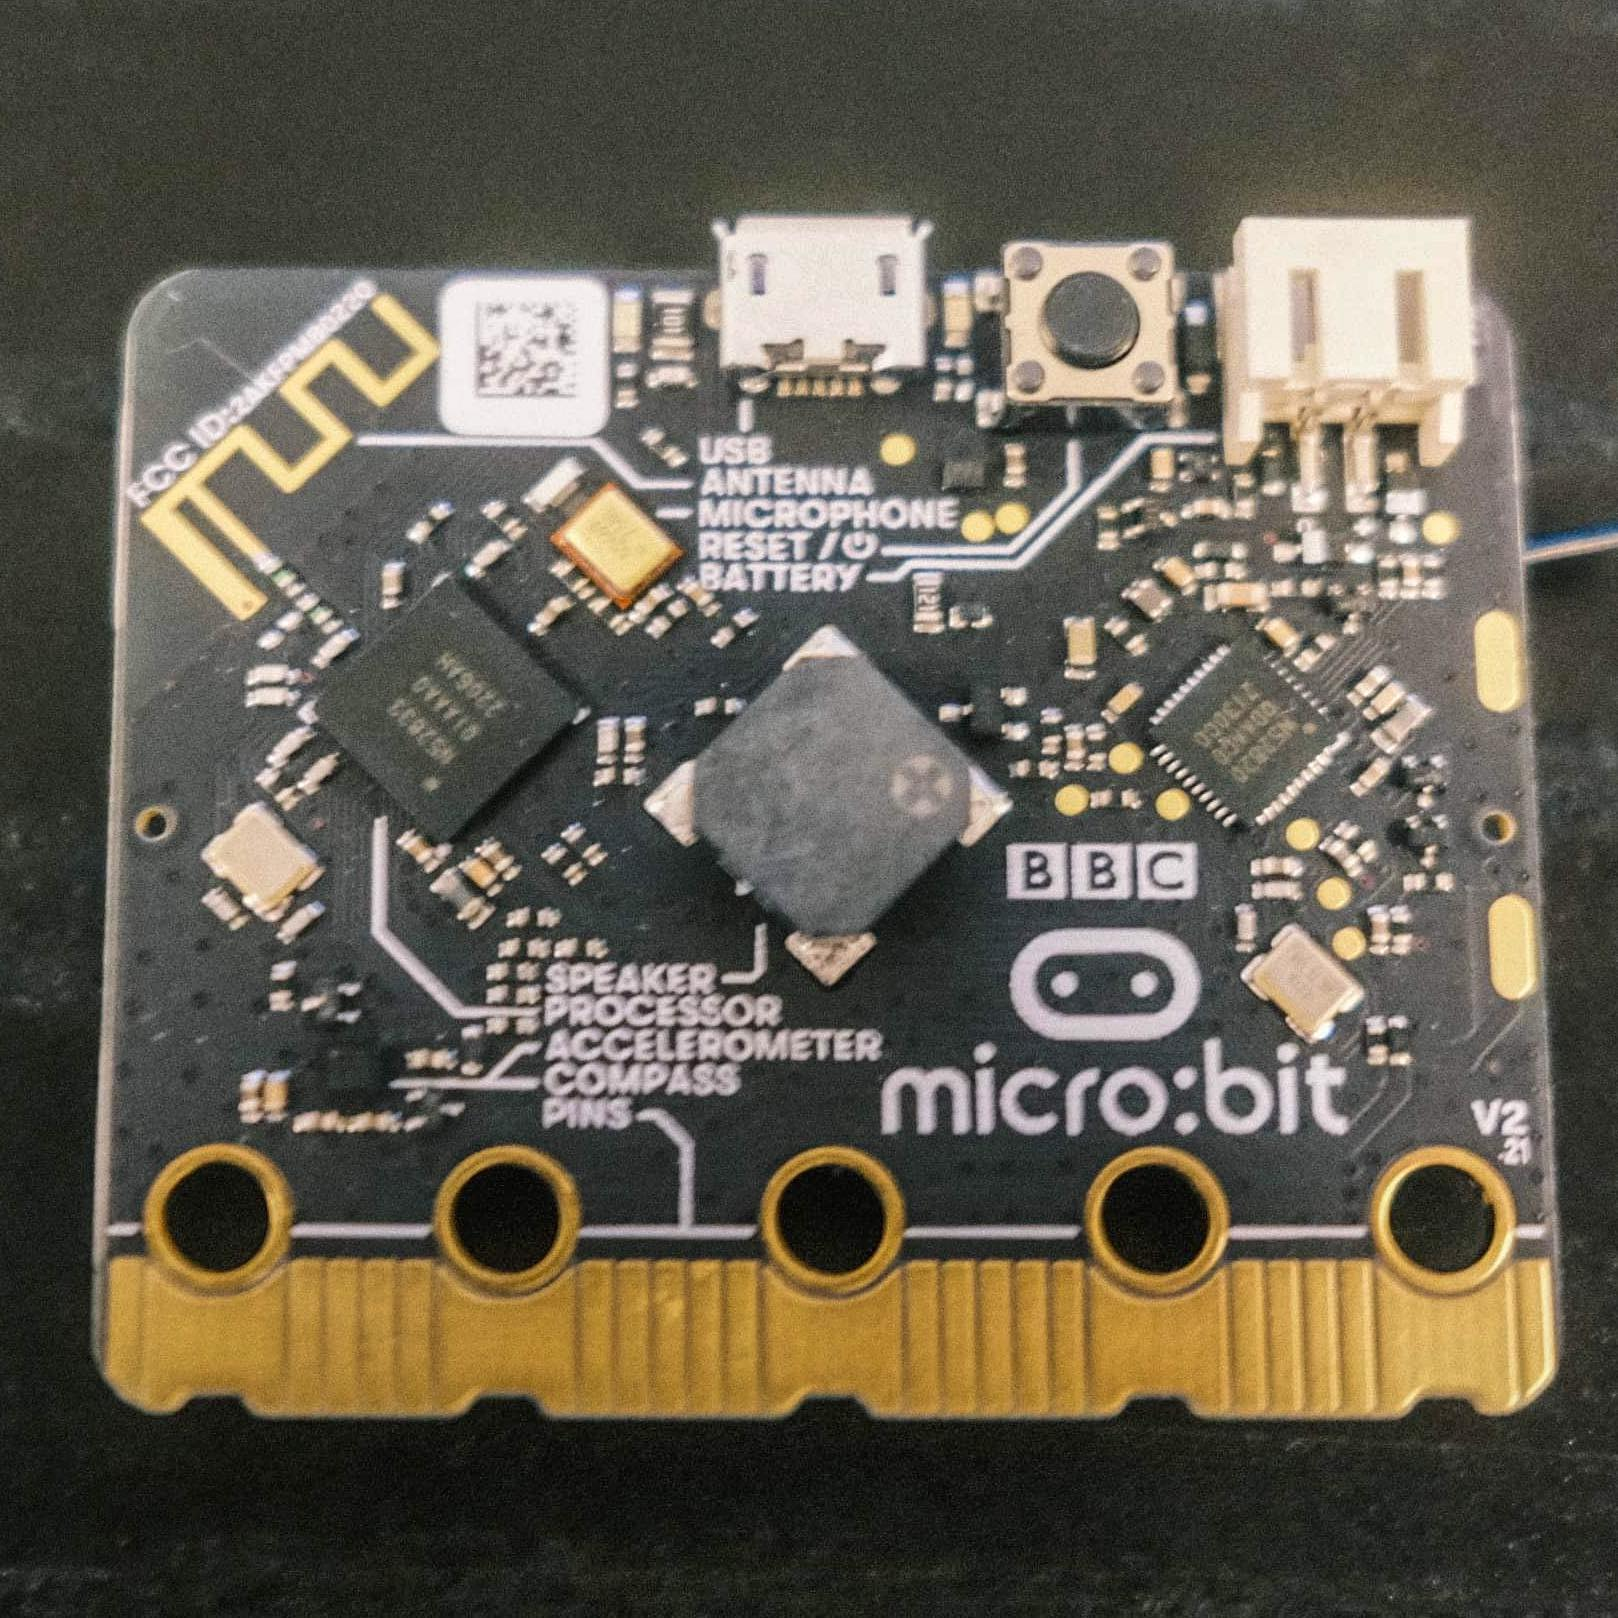
\includegraphics[width=.8\linewidth]{figures/microbit1}
        \caption{Baksiden med sensorer}
        \label{fig:inclu}
    \end{subfigure}%
    \begin{subfigure}{0.5\textwidth}
    \centering
        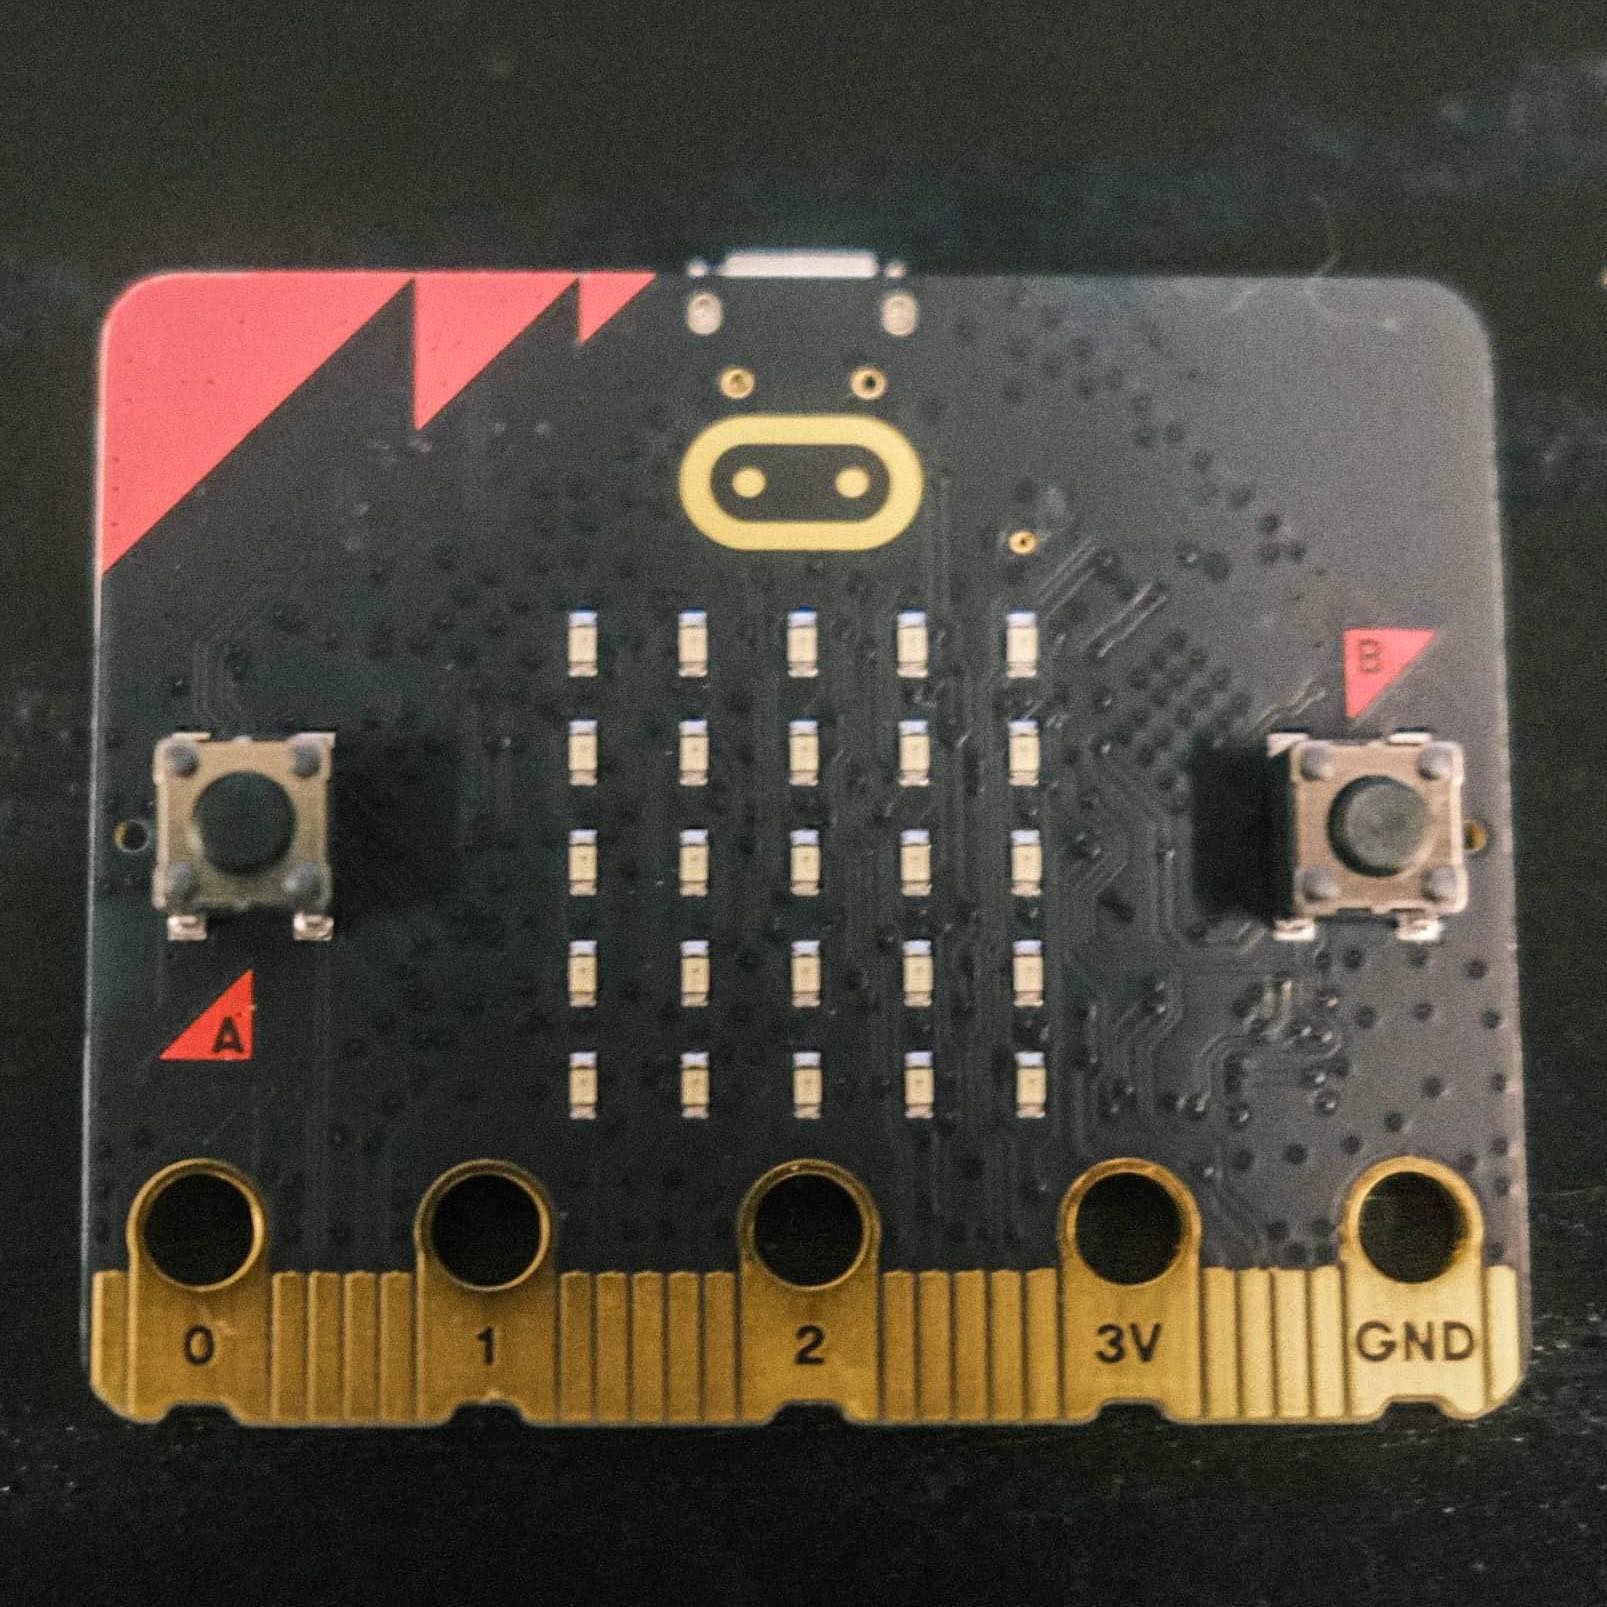
\includegraphics[width=0.8\linewidth]{figures/microbit2}
        \caption{Forsiden med led-lys og knapper}
        \label{fig:deform}
    \end{subfigure}
    \caption{micro:bit-en brukt i mikrokontroller labben.}
    \label{fig:micro:bit}
\end{figure}



Under webgrensesnittet i abstraksjonsnivåstigen ligger micro:bit {DAL} (\textbf{D}evice \textbf{A}bstraction \textbf{Layer}). Denne kan programmeres med MicroPython eller JavaScript. Ulempen med micro:bit DAL programmering er at mye av minnet blir brukt opp. MicroPython vil for eksempel legge beslag på omlag 14 kB, som er ganske mye ettersom micro:bit-en bare har totalt 128 KB.

For å få en mer effektiv bruk av ressursene er det også mulig å benytte seg av \verb|C++|, eksempelvis med ARM sin mbed-platform. Allikevel vil de fleste detaljene om hvordan kortet fungerer være abstrahert bort, også på dette nivået.

For å få en bedre forståelse for hvordan de lagene henger sammen kan man derfor gå forbi DAL-en og programmere mikrokontrollerens registre direkte. Dette gjøres med \verb|C|, som er det laveste abstraksjonsnivået man kan få til, uten å gå over til Thumb - som er prosessorens instruksjonssett. Prosessoren på kortet er en ARM Cortex M4, som er integrert inn i en Nordic Semiconductor nRF52833 SoC.

\begin{figure}[H]
    \centering
        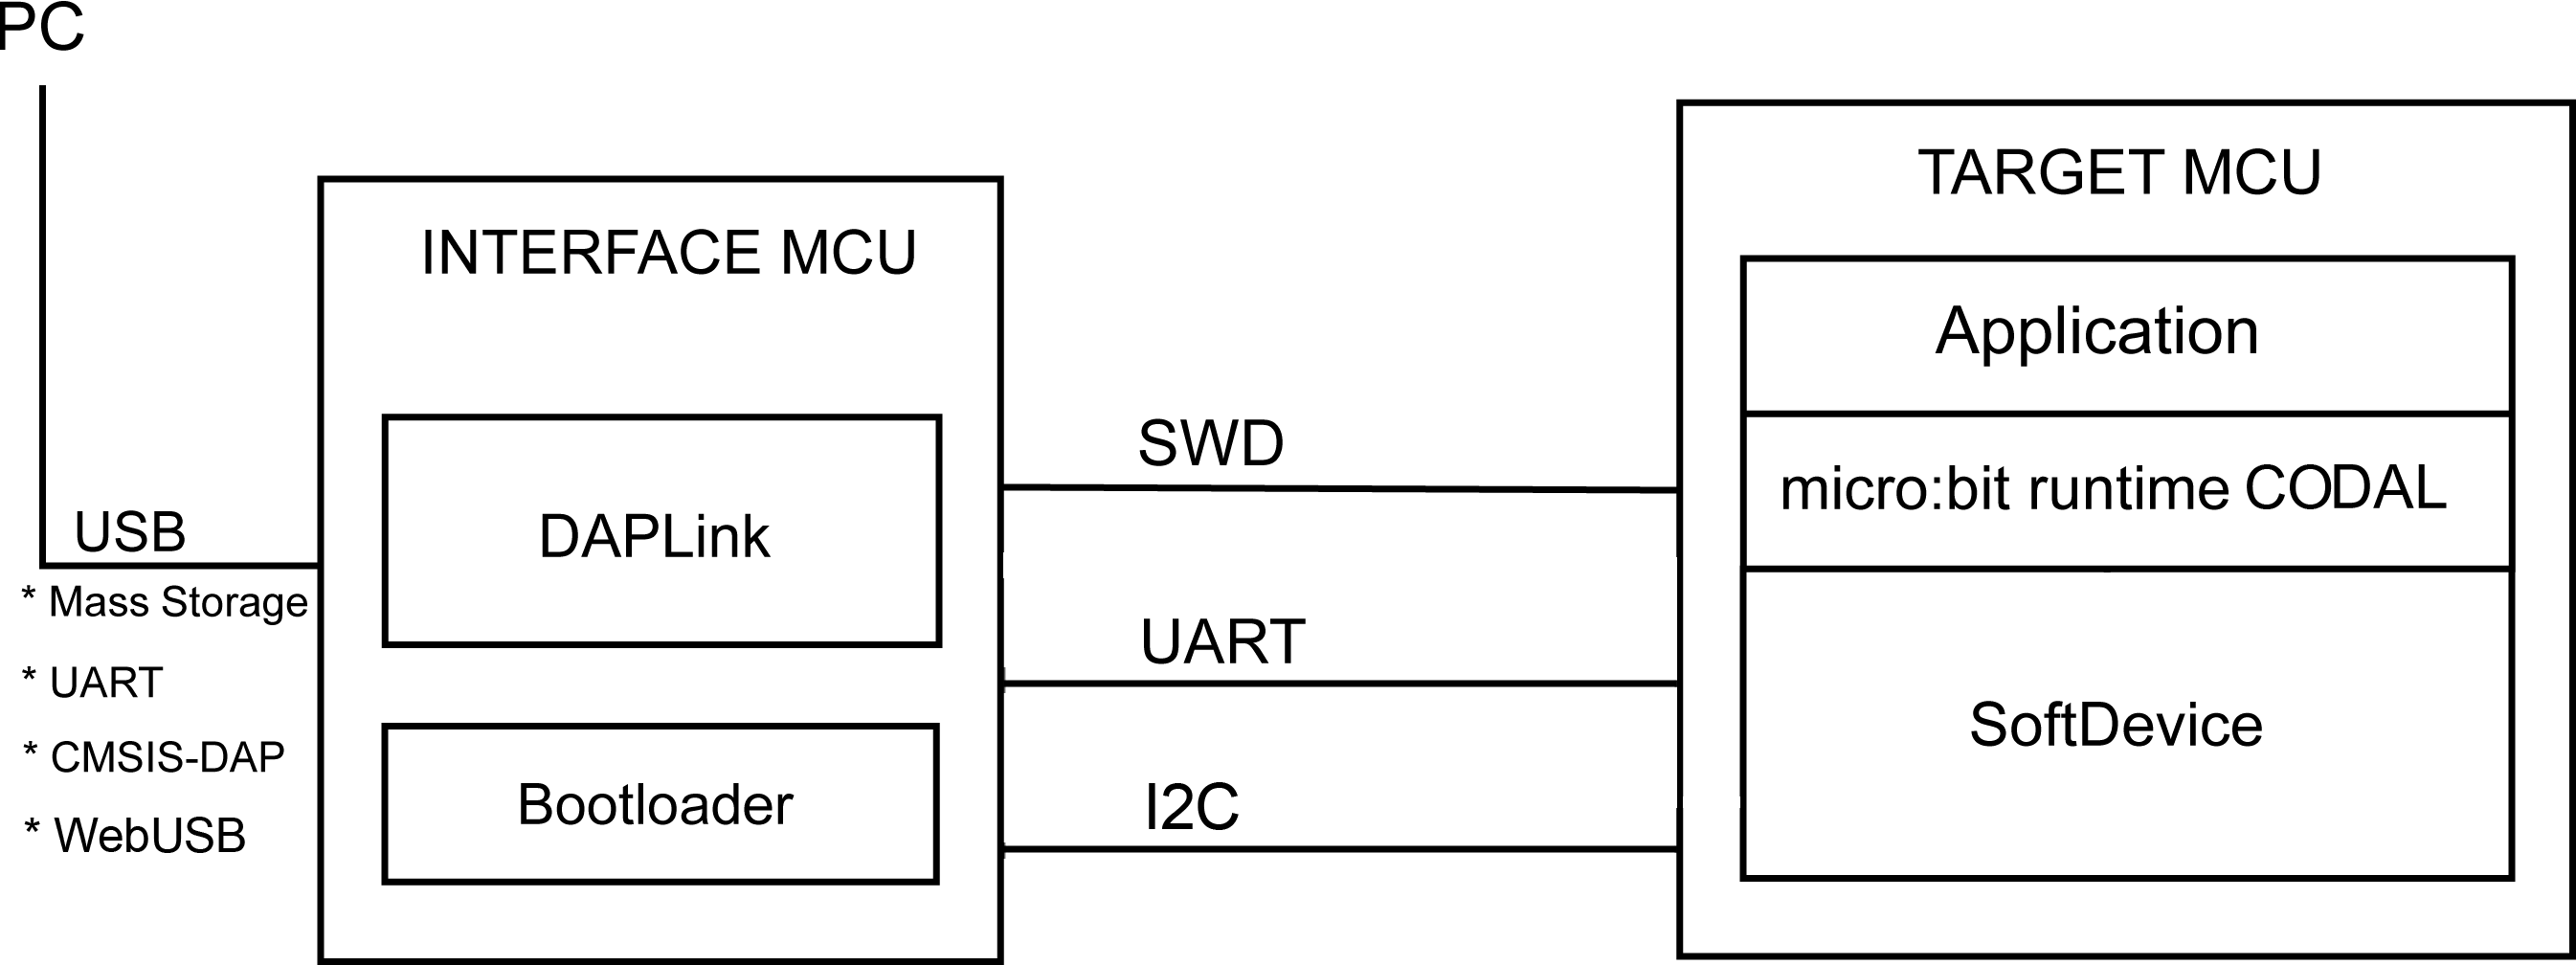
\includegraphics[width=0.8\linewidth]{figures/microbit_interface.png}
        \label{fig:deform}
    \caption{micro:bit-en har to mikrokontrollere.}
    \label{fig:micro:bit-interface}
\end{figure}

Hvis du ser nøye etter på baksiden av micro:bit-en, vil du legge merke til at den har to chipper: en større merket med N52833, og en mindre merket med N52820. Micro:bit-en har nemlig to mikrokontrollere, også kalt {MCU}er (\textbf{M}icro\textbf{c}ontroller \textbf{U}nit): En som kjører programvare utelukkende for å programmere og feilsøke hovedchippen, og en som faktisk kjører koden vår. Vi skiller mellom dem med ved navnene "Target" og "Interface" (se figur \ref{fig:micro:bit-interface}). Når du kobler til micro:bit-en til en datamaskin, vil datamaskinen kommunisere med interface MCUen og oppdage den som USB-lagringsenhet. Programvaren \href{https://tech.microbit.org/software/daplink-interface/}{DAPLink} gjør det da mulig å laste over ferdigkompilerte programmer over til USB-enheten, og vil programmere target MCUen for oss. Det er denne metoden vi skal bruke til å programmere micro:bit-en i denne laben. De som er ekstra interesserte kan se appendiks\ref{app:Debugging} for alternative metoder for både debugging og programmering. 

\section{Praktisk rundt filene}

I denne laben får dere utlevert noen \verb|.c| og \verb|.h|-filer. Egne tabeller under hver oppgave lister opp alle filene som kommer med, samt litt informasjon om dere skal endre på filene eller om dere skal la dem forbli i løpet av oppgaven.


\section{Introduksjon - Praktisk rundt laben}


I denne laben brukes ARM GCC som verktøykjeden for programmering av micro:bit-en. Denne typen verktøykjede kalles åpen kilde, og er helt uten begrensninger. Dette er i motsetning til andre IDE-er (\textbf{I}ntegrated \textbf{D}evelopment \textbf{E}nvironments) for utvikling av tilpassede datasystemer som vanligvis koster en del. 

For å gjøre denne laben litt lettere blir det lagt til en \verb|Makefile| for hver oppgave. Denne vil bygge kildekoden, sette opp riktig minnefordeling på prosessoren, og deretter skrive koden til den. I tillegg blir det også utdelt en undermappe ved navn \verb|.buid_system|. Denne inneholder det som skal til for å få koden til å kjøre på micro:bit-en. 

Det er ikke meningen at \verb|.build_system|-mappen skal endres, men om man vil forstå hvordan koden henger sammen med hva som fysisk skjer på micro:bit-en, er det bare å ta en titt.

Målet med denne laben er at dere først og fremst skal ha det gøy. Siden dere får ta med micro:bit-en hjem etter faget, så er tanken at dere skal lære nok i denne laben slik at eventuelle hobbyprosjekter kan implementeres direkte på micro:bit-en. I tillegg skal dere lære dere hvordan man leser datablad. Det å kunne lese datablad er veldig viktig dersom man har lyst til å jobbe med mikrokontrollere senere, men også til eksamen.


\subsection{Makefile}

I denne laben blir det gitt ut ferdige \verb|Makefiler|. Slik som i \verb|Makefile|-øvingen, kaller man \verb|make| fra et terminalvindu i samme mappen som \verb|Makefilen| for å kompilere \verb|C|-koden. Dette vil genere en \verb|.hex|-fil som mikrokontrolleren kan kjøre i \verb|.build_system|-mappen. I tillegg til \verb|make|, har denne \verb|Makefilen| også tre andre mål; \verb|make debug| vil kompilere \verb|C|-koden med debug-flagg for feilsøking av programmet, \verb|make erase| vil slette minnet til mikrokontrolleren, mens \verb|make clean| vil slette ferdigkompilert kode og \verb|hex|-filen fra datamaskinen. For å faktisk overføre \verb|hex|-filen over i programminnet til mikrokontrolleren går man først inn i \verb|.build_system|-mappen, også dragger man \verb|hex|-filen over til \verb|MICROBIT|-mappen som representerer micro:bit-en. Denne mappen burde komme opp som en enhet på datamaskinen når man kobler micro:bit-en med USB på datamaskinene på sanntidssalen. Alternativt kan en kjøre målet \verb|make load| for å laste over \verb|hex|-filen til micro:bit-en. Denne metoden krever at man har laster over en \verb|.hex|-fil via drag-and-drop-metoden først for å skrive over programmet micro:bit-en kommer med.

\subsection{Programmeringstaktikk}

For å sette ønskede registre på nRF52833-en, burde man bruke et kjent triks fra \verb|C|-programmering. Dette innebærer at man lager \verb|struct|s, som dekker nøyaktig det minnet man ønsker å tukle med - for dermed å \textit{typecaste} en peker til starten av minnet inn i \verb|struct|-en. Dette gjør det mulig å endre \verb|struct|-ens medlemsvariabler, og samtidig skrive til det underliggende minnet.

Dette er definisjonen på \textit{memory mapped IO}; man gjør endringer som i software ser ut som vanlige lese- og skriveoperasjoner i samme minnerom som resten av programmet, men i bakgrunnen peker deler av dette minnet til registre hos perifere enheter. Dette er i kontrast til \textit{port mapped IO}, hvor egne instruksjoner brukes for å gjøre operasjoner i et disjunkt minneområde fra programmet (se forøvrig forelesningene for mer om dette tema).

\subsection{Datablad}


Tilpassede datasystemer er forskjellige fra vanlige datasystemer, fordi de er skreddersydde for en spesifikk oppgave. Ofte må de fungere med begrensede ressurser, og gjerne over lang tid kun drevet av et knappecelle-batteri. Derfor må man som oftest glemme en del generelle ting som gjelder uavhengig av plattform, og fokusere på ting som kun gjelder plattformen man arbeider på. Det er her datablad kommer inn.

Datablader er essensielt dersom man vil være god på å programmere tilpassede datasystemer. For micro:bit-en, gjelder \texttt{nRF52833 Product Specification} (denne finner dere i samme mappe som denne \verb|.pdf|-en). Det er viktig å bruke denne flittig, ettersom den gir en nokså kortfattet dokumentasjon som beskriver nøyaktig arkitekturen til datasystemet som blir brukt.

Det er lurt å sjekke ut appendiks \ref{app:datablad} for en kjapp innføring i hvordan man leser og bruker databladet til micro:bit-en i kontekst av memory mapped IO før dere slenger dere løs på oppgavene. 




\subsection{Førstegangsoppsett}


Før man bruker micro:bit-en må man laste ned redskapene som trengs for å programmere en micro:bit i Ubuntu. Det eneste som trengs før dere kan begynne egentlig er kompilatoren. Denne burde allerede være installert, men dersom den ikke er det så kan den installeres med følgende kommando:


\verb|sudo apt install gcc-arm-none-eabi|

Kompilatoren vi skal bruke er GCC for ARM. På Linuxmaskiner finnes
denne utvidelsen for GCC gjerne i systempakkelageret allerede. 

\subsection{Strategier for feilsøking}
Å feilsøke, også kalt å \verb|debugge|, mikrokontrollere kan være utfordrende på grunn av mangelen på interaktive verktøy og begrensede ressurser tilgjengelig på mikrokontrollere. Selv om kompilatoren luker ut de fleste feil, er man fremdeles utsatt for logiske feil. Det finnes imidlertid to vanlige metoder som kan brukes til å feilsøke program som kjører på tilpassede datasystemer som du kan lære om i denne laben. En av disse metodene er \verb|Seriell debugging| som innebærer å koble en seriell kabel (se oppgave \ref{sec:4-oppgave-UART}) mellom micro:bit-en og datamaskinen for å bruke et seriell terminalprogram for å skrive ut feilsøkingsdata fra micro:bit-en. 

Den andre metoden er å bruke et debuggingsprogram som kommuniserer med Interface MCUen (se figur \ref{fig:micro:bit-interface}). Denne metoden blir beskrevet i appendiks \ref{app:Debugging}. Selv om det ikke er noe krav om å bruke noen av disse metodene for å feilsøke oppgavene, anbefaler vi å undersøke dem av egen interesse.


\end{alphasection}



\setcounter{section}{0}
